\chapter{Аппаратная платформа и алгоритм проведения измерений}
	
Управляющее устройство реализовано на базе ПЛИС, так как есть необходимость разрабатывать 
специфические аппаратные модули.

На основании требований к количеству логических ячеек в ПЛИС и необходимой обвязке студентом Владиславом
Михайловским была разработана структурная схема устройства (\firef{fig:scheme-struct}) и печатная плата (\firef{fig:pcb}).

В качестве аппаратной платформы УУ (управляющее устройство) выступает ПЛИС серии
LittleBee китайского производителя Gowin Semiconductor -- GW1N-UV9QN88C6/I5.\\

\noindent Данная ПЛИС имеет следующие характеристики:\\


\begin{itemize}
	\item количество логических блоков LUT4 -- 8640 шт.
	\item количество триггеров -- 6480 шт.
	\item объём FLASH -- 408 Кбит
	\item количество блоков BSRAM -- 26 шт.
	\item объём блоков SRAM -- 468 Кбит
	\item количество блоков PLL (ФАПЧ) -- 2 шт.
	\item напряжение питания ядра -- 1.8–3.3 В
	\item количество доступных для пользователя выходов I/O -- 77
	\item среди них дифференциальных пар -- 19\\
\end{itemize}

\begin{figure}[ht!] 
	\center
	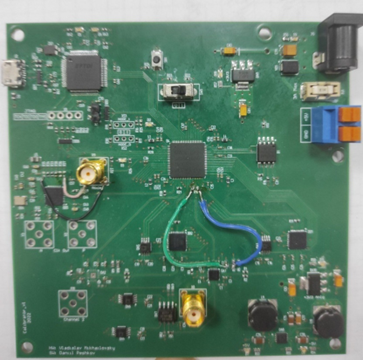
\includegraphics {my_folder/images//pcb}
	\caption{Печатная плата устройства} 
	\label{fig:pcb}  
\end{figure}

\begin{figure}[ht!] 
	\center
	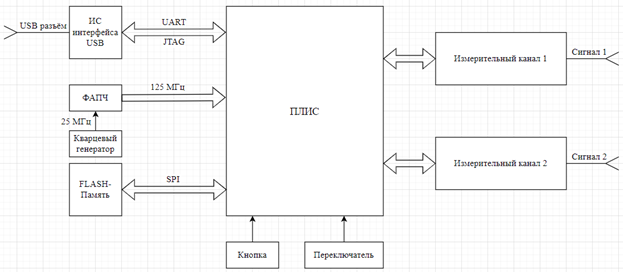
\includegraphics {my_folder/images//scheme_struct}
	\caption{Структурная схема устройства} 
	\label{fig:scheme-struct}  
\end{figure}

К УУ подключаются два измерительных канала, которыми необходимо управлять для проведения измерений.
ПЛИС тактируется высокостабильным тактовым сигналом с частотой 125 МГц. Связь с устройством верхнего уровня
осуществляется через FTDI чип FT2232H[5].

Перед разработкой УУ необходимо определить ОУ (объект управления), которым предстоит управлять.

\FloatBarrier

\section{Измерительный канал}

На \firef{fig:ch-func} приведена функциональная схема одного из измерительных каналов.

\FloatBarrier

\begin{figure}[ht!] 
	\center
	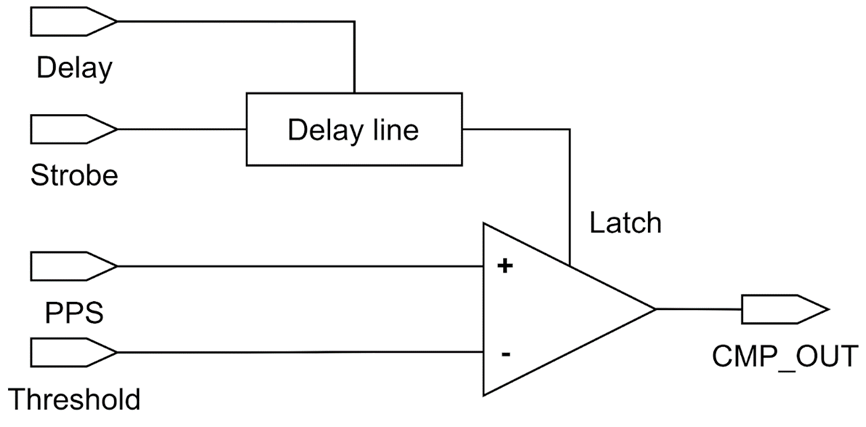
\includegraphics [scale=0.3] {my_folder/images//ch_func}
	\caption{Функциональная схема измерительного канала} 
	\label{fig:ch-func}  
\end{figure}

\FloatBarrier


\begin{itemize}[label={}]
	\item SPI (Serial Peripheral Interface) –- интерфейс для задания напряжения на ЦАП\_X/Y
	\item Подстройка/настройка –- сигналы управления ПЛЗ. Задают величину, на которую происходит задержка сигнала строба
	\item Строб –- сигнал, при получении которого компаратор фиксирует текущее значение своего выхода и удерживает его
	\item ЦАП\_X –- Цифро-Аналоговый Преобразователь. Используется для задания напряжения, управляющего подстройкой задержки ПЛЗ
	\item ЦАП\_Y -- Цифро-Аналоговый Преобразователь. Используется для задания величины порогового напряжения сравнения для компаратора
	\item ПЛЗ –- программируемая линия задержки. Используется для изменения задержки распространения строба на заданную величину
	\item Компаратор –- устройство, производящее сравнение входного Сигнала PPS и пороговым значением сравнения
	\item Пороговое напряжение сравнения –- задаваемое ПЛИС значение напряжения, с которым происходит сравнение
	\item PPS –- входной синхросигнал от калибруемого устройства
\end{itemize}

\section{Алгоритм проведения измерений}

Разрабатываемое устройство, помимо узкоспециализированного применения для измерения разности фаз синхросигналов
калибруемых устройств, также может работать в режиме стробоскопического осциллографа общего назначения.

\subsection{Режим измерения разности фаз}

Для определения разности фаз сначала находится фаза синхросигнала опорного устройства (то, от которого тактируется калибратор). Для этого
на ЦАП\_У устанавливается пороговое напряжение, характерное для используемого стандарта ввода-вывода
измеряемого сигнала. Затем, увеличивая значение задержки, находится такое,
при котором на выходе компаратора на втором канале будет логическая единица. Для нахождения разности фаз ($ skew_{PPS} $) (\firef{fig:meas-skew})
необходимо умножить установленный код на линии задержки на шаг изменения задержки.

\FloatBarrier

\begin{figure}[ht!] 
	\center
	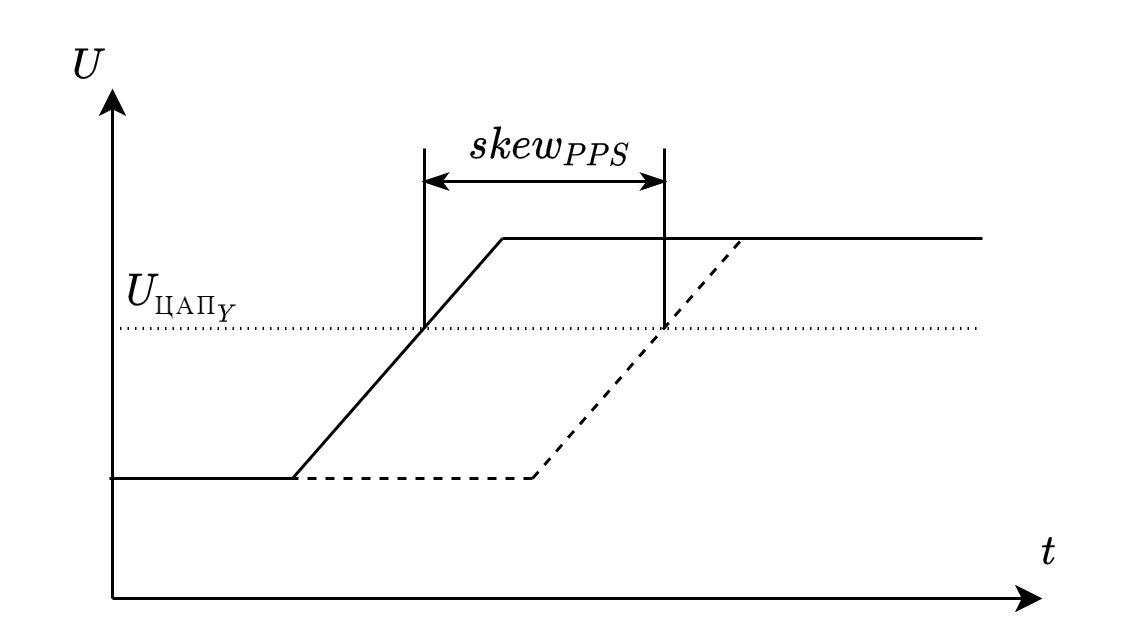
\includegraphics [scale=0.4] {my_folder/images//measure_skew}
	\caption{Измерение разности фаз} 
	\label{fig:meas-skew}  
\end{figure}
 
\FloatBarrier

\subsection{Режим стробоскопического осциллографа}

Перед началом проведения измерения необходимо определить частоту измеряемого сигнала, и начать генерировать стробы с той же частотой.
Стробы блокируют текущий выход компаратора, и на его выходе остаётся результат сравнения в момент прихода строба.
При помощи изменения задержки можно сдвигать момент прихода стробы, тем самым сдвигая измеряемую точку по оси OX.

Для поиска значения напряжения в измеряемой точке необходимо изменять пороговое напряжение сравнения на компараторе. 
Наблюдая изменения выхода компаратора, в зависимости от значения порогового напряжения, можно судить о том, найдено ли значение
в измеряемой точке.

\begin{figure}[ht!] 
	\center
	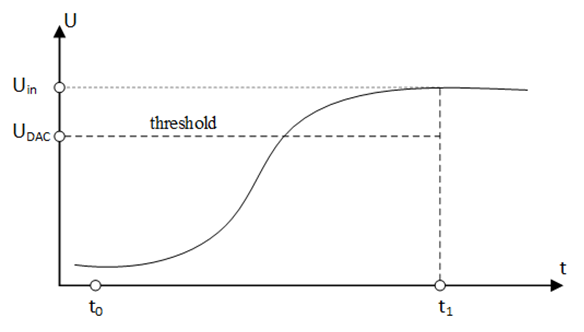
\includegraphics {my_folder/images//meas_alg}
	\caption{Снятие осциллограммы сигнала} 
	\label{fig:meas-alg}  
\end{figure}

На \firef{fig:meas-alg} приведён пример измерения. 
$ t_{0} $ -- точка от которой измеряется сигнал (момент прихода строба),
$ t_{1} $ -- измеряемая точка (момент прихода задержанного строба на компаратор).
Временной отрезок $ [t_{0}$ , $ t_{1}] $  настраивается линией задержки.
Если в момент защёлкивания на выходе компаратора логическая единица, значит измеряемое напряжение выше,
чем пороговое. Перед приходом следующего строба пороговое напряжение повышается.
Так продолжается до тех пор, пока на выходе компаратора не будет логического нуля.
В таком случае мы считаем, что измеряемая точка имеет значения напряжение равное пороговому.

Затем увеличивается значение задержки и начинается поиск значения напряжения в следующей точке.

\section{Пороговое напряжение сравнения}

Для задания порогового напряжения используется ЦАП AD5662 от Analog Devices.
AD5662 -- 16-битный ЦАП с гарантированной точностью 12 бит.

С опорным напряжением 3.3 В, шаг изменения напряжения -- $ \frac{3.3}{2^{16}} \approx 50 $ мкВ (если не учитывать нелинейность задания напряжения).
Для задания напряжения используется интерфейс SPI (\firef{fig:dac-interface}).

\FloatBarrier

\begin{figure}[ht!] 
	\center
	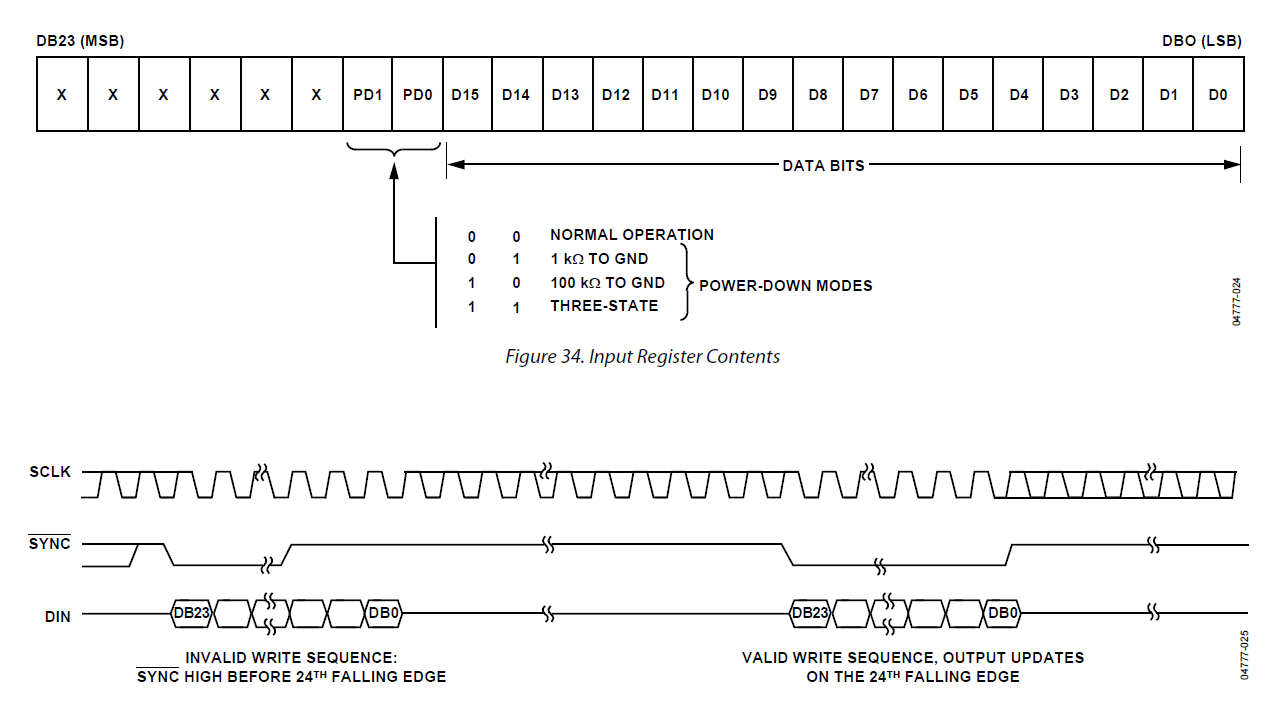
\includegraphics [scale=0.5] {my_folder/images//dac_interface}
	\caption{Интерфейс взаимодействия с AD5662} 
	\label{fig:dac-interface}  
\end{figure}

\FloatBarrier

При напряжении питания 3.3 В максимальная частота сигнала SCLK -- 20 МГц. Максимальное время установки
выходного напряжения -- 10 мкс (обычно 8 мкс). Описание используемого ЦАП приведено в документации[3].

\section{Линия задержки}

Для задержки строба используется программируемая линия задержки SY100EP196V пр-ва Microchip.
Задержка задаётся 10-битным цифровым кодом с шагом $ \approx $ 10 пс (\firef{fig:dline-code}).
Так же есть аналоговый вход FTUNE, которым можно точнее точнее подстраивать
задержку в диапазоне 30 пс (\firef{fig:dline-ftune}) (на данный момент не используется).

\FloatBarrier

\begin{figure}[ht!] 
	\center
	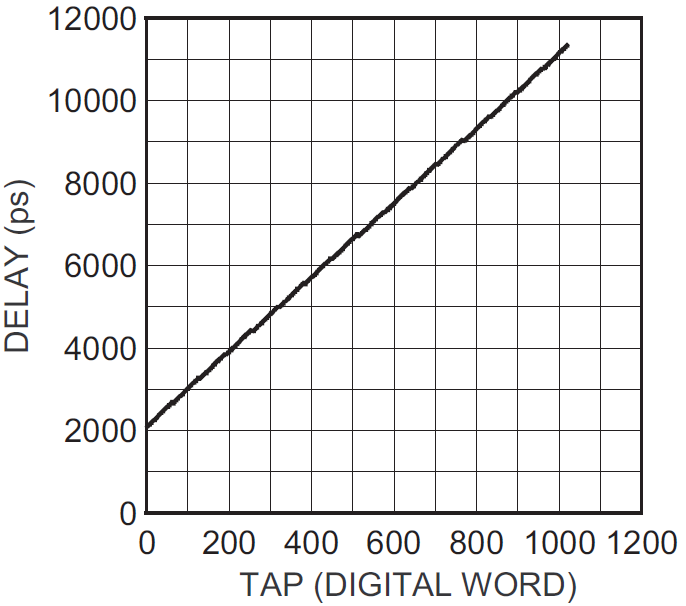
\includegraphics [scale=0.6] {my_folder/images//dline_code}
	\caption{Задержка, задаваемая цифровым входом} 
	\label{fig:dline-code}  
\end{figure}

\begin{figure}[ht!] 
	\center
	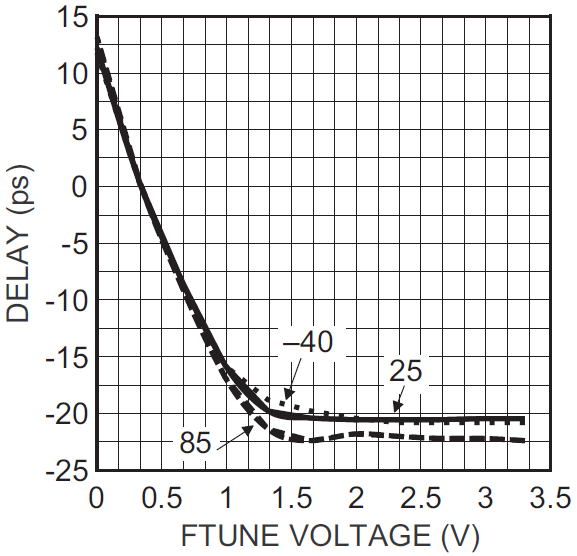
\includegraphics [scale=0.6] {my_folder/images//dline_ftune}
	\caption{Подстройка задержки через аналоговый вход FTUNE} 
	\label{fig:dline-ftune}  
\end{figure}

\FloatBarrier

Описание используемой программируемой линии задержки приведено в документации[12].

\section{Компаратор}

Для сравнения используется компаратор ADCMP582 от Analog Devices.
Основным параметром, который необходимо учесть является $ t_{PL} $ (\firef{fig:cmp-wave}).

\begin{figure}[ht!] 
	\center
	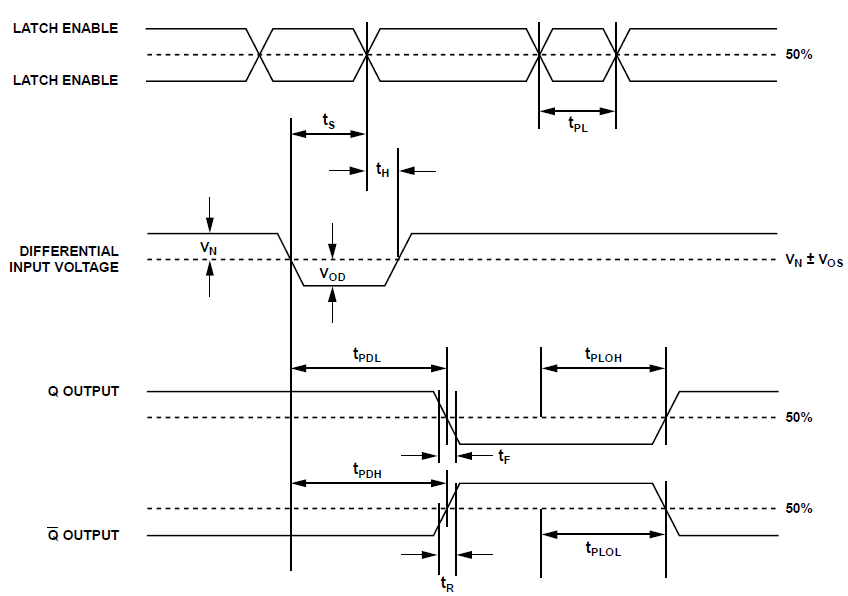
\includegraphics [scale=0.7] {my_folder/images//cmp_wave}
	\caption{Временная диаграмма ADCMP582} 
	\label{fig:cmp-wave}  
\end{figure}
\FloatBarrier

$ t_{PL} $ -- минимальное время, в течение которого вход защёлки (Latch Enable) должен быть высоким, чтобы результат сравнения попал на выход компаратора.

Описание использованного компаратора приведено в документации[2].
\newpage